%%%%%%%%%%%%%%%%%%%%%%%%%%%%%%%%%%%%%%%%%%%%%%%%%%%%%%%%%%%%%%%%%%%%%%%%%
% This file is part of the LaTeX sources of the OMDoc 1.3 specifiation
% Copyright (c) 2006 Peter Jansen
% This work is licensed by the Creative Commons Share-Alike license
% see http://creativecommons.org/licenses/by-sa/2.5/ for details
\svnInfo $Id: report.tex 8453 2009-08-04 09:58:26Z kohlhase $
\svnKeyword $HeadURL: https://svn.omdoc.org/repos/omdoc/branches/omdoc-1.3/doc/spec/projects/omdocmode/report.tex $
%%%%%%%%%%%%%%%%%%%%%%%%%%%%%%%%%%%%%%%%%%%%%%%%%%%%%%%%%%%%%%%%%%%%%%%%%

\section{An Emacs mode for editing OMDoc Documents}
\begin{project}{omdocmode}{http://www.cs.cmu.edu/~ccaps}
\pauthors{Peter Jansen}
\pinstitute{School of Computer Science, Carnegie Mellon University}
\end{project}

We describe an {\emacs} major mode for editing {\omdoc} documents, developed by the {\scsys{Course Capsules}}
project group at the CMU School of Computer Science.  This mode extends the {\emacs}
editor~\cite{Stallman:em02} with functionality intended to help visualize, edit, and
create documents written in {\omdoc} format.

The mode is part of the {\omdoc} distribution (see {\mysecref{distribution}}), it is
provided under the conditions specified in the Library Gnu Public License~\cite{LGPL}.

\subsection{Introduction}

The CCaps project has developed tools to convert legacy materials written in a variety of
formats ({\scsys{PowerPoint}}, {\mathematica}, etc.)  into the {\omdoc} format (see
{\mysecsref{cpoint}{nb2omdoc}}). In many cases the output generated by such tools needs to
be post-processed or otherwise modified.

To this end, a user must open the file, read and understand its contents and perform the
appropriate modifications.  Though an {\omdoc} document is a regular text file, most of
its content consists of markup, which is hard to read and tedious to type.  It is
therefore important to support the user with tools that make a document easier to read and
modify, either in the form of a separate editor, or as an extension of an existing editor.

One approach to this is to build a {\emph{visual {\omdoc} editor}}, which presents the
document in a form resembling conventional mathematical documents (i.e., without showing
the markup explicitly, and with appropriate formatting for mathematical formulae), and
offers the user functionality to modify or annotate its content.

While this is ideal for user understanding of document content, it presupposes
consistent syntactic correctness, makes it more difficult to inspect or change
markup directly, and may present challenges as to resolving user action
ambiguities.

We have taken this approach in the {\cpoint} and {\mathematica} add-ins (see
{\mysecsref{cpoint}{nb2omdoc}}). But we also wanted a tool that would maintain full
control of all the textual information, while offering support for readability and editing
functionality.  We chose for this tool to extend the {\emacs} editor~\cite{Stallman:em02},
which lends itself very well to this task (as well as being the editor for general use for
several of our group).

\subsection{{\omdoc} mode functionality}

We now look at the different categories of
functionality in slightly more detail.

\paragraph{Visualization}
is currently provided by the use of the {\emacs} {\emph{font-lock}} mechanism to give
different categories of tags and content different fonts and colors to make them easily
recognizable.  Element categories currently recognized correspond to the {\omdoc} 1.2
modules: Document structure, Math, Theories, Auxiliaries, Presentation, {\openmath}, and
the {\indextoo{Dublin Core}} elements.

A customizable {\emph{indentation function}} allows for intelligible layout, which is
helpful both in hand-coding and the editing of the output of a legacy transformation
process.  There are key bindings for line, region, and enclosing element indentation.

\paragraph{Editing}
Functionality consists mainly of automated insertion of {\emph{templates}} for each of the
{\omdoc} elements, both via mode-dependent menu options and key bindings, grouped by
element category (the same categories as given above).

The template insertion mechanism is based on {\snippet{tempo.el}}, which allows for the
maintenance of a {\emph{list of insertion points}} the user can navigate in between to
supply or change the values of certain attributes.

The main function currently available for completing incomplete elements is the equivalent
of the standard {\snippet{electric-/}} function.  We are planning to add several other
completion functions in the near future (for tags, tag sets, attribute names, and symbol
and theory names).

The mode also provides for {\emph{validation}}: either internally (as a simple local
syntax check to check well-formedness) or externally (via an external xml validation
validation engine).  Internal validation builds an abbreviated parse tree, and highlights
discrepancies, suggesting possible modifications of insertions of element opening or
closing tags.  External validation runs an external xml validation engine ({\rxp} or
{\nsgmls}, depending on the configuration variables), and shows the output in a separate
buffer.

\begin{myfig}{skeleton}{Opening a new Buffer in {\omdoc} Mode}
  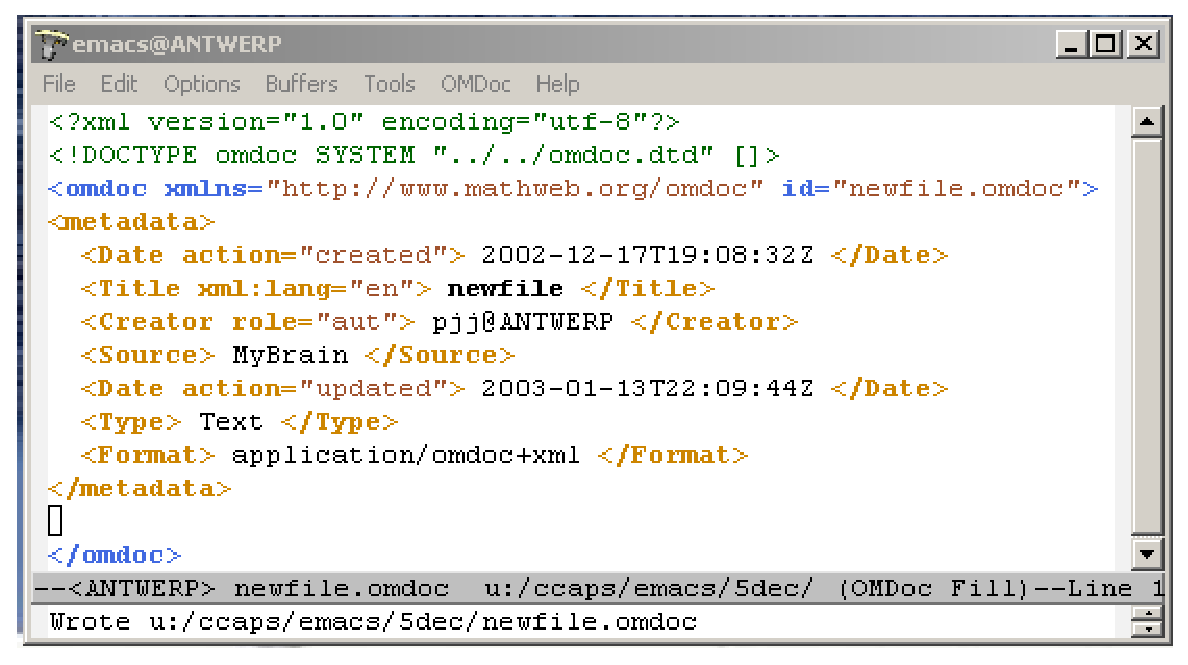
\includegraphics[width=9cm]{projects/omdocmode/omdoc2c}
\end{myfig}

\paragraph{Document creation}
is supported by automatic insertion of a basic {\emph{{\omdoc} skeleton}} in new buffers
as well as a {\emph{time-stamp updating}} mechanism and some smaller functions that extract
information from the user's environment variables to supply information for some of the
metadata slots (see the example in {\myfigref{skeleton}} below).

\subsection{Examples}

We illustrate some of the above by means of a few screen shots.  The example in
{\myfigref{menu}} is taken while editing a document that was semi-automatically generated
from part of a {\mathematica} notebook~(\cite{Sutner:cmnto04}).  Here, the user has
already run an automated indentation function, for example by activating
{\snippet{omdoc-indent-enclosing-main}} by typing {\snippet{C-c C-q}}, and is now about to
use the {\omdoc} menu to enter a new construct.


\begin{myfig}{menu}{Editing an {\omdoc} Document}
  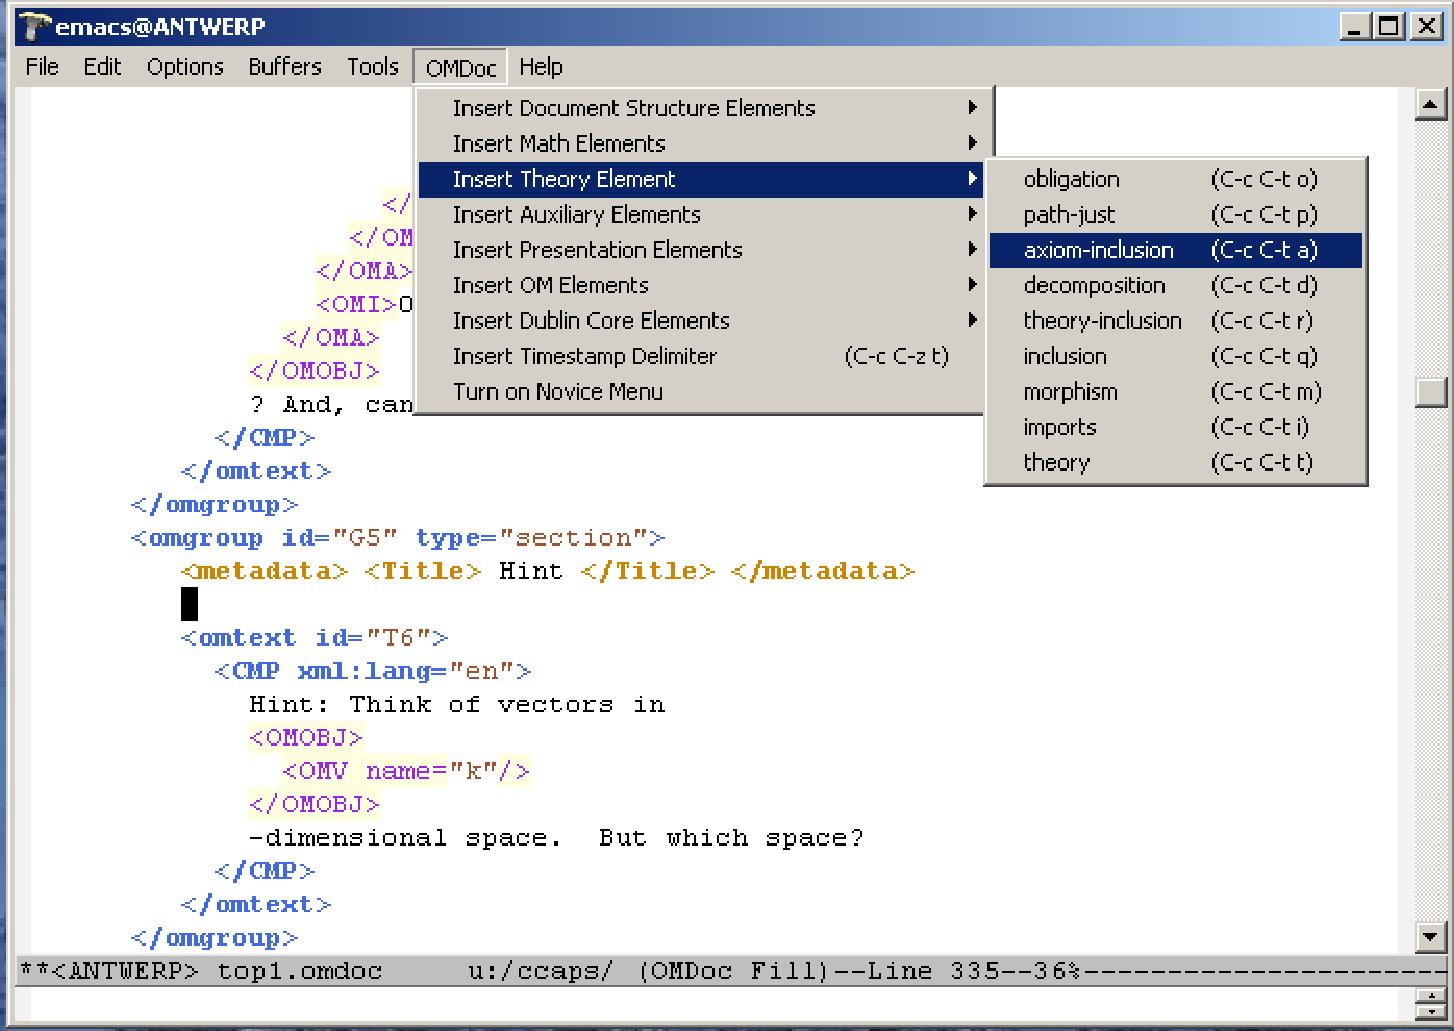
\includegraphics[width=9cm]{projects/omdocmode/omdoc1c}
\end{myfig}

After this operation, which could also have been performed by typing the key sequence
{\snippet{C-c C-t a}}), {\emacs} inserts the following text at the point (i.e. cursor
position).
\begin{lstlisting}
<axiom-inclusion xml:id="" to=""> </axiom-inclusion>
\end{lstlisting}

The second example shows the skeleton template that is automatically inserted when the
user opens a new file: {\myfigref{skeleton}}.  Note that the file name has been used as id
and title automatically, and the user's address appears in the Author field.  Timestamps
are inserted in Date fields for both creation and update, and the latter is adjusted
automatically every time changes are saved to the file.

%%% Local Variables: 
%%% mode: latex
%%% TeX-master: "../../omdoc"
%%% End: 

% LocalWords:  omdocmode el CCaps cpoint nb omdoc metadata
